%% LyX 1.5.5 created this file.  For more info, see http://www.lyx.org/.
%% Do not edit unless you really know what you are doing.
\documentclass[a4paper,twoside,czech,czech,openright,cleardoubleempty,BCOR10mm,DIV11]{scrreprt}
\usepackage[T1]{fontenc}
\usepackage[utf8]{inputenc}
\usepackage{array}
\usepackage{longtable}
\usepackage{varioref}
\usepackage{wrapfig}
\usepackage{fancybox}
\usepackage{calc}
\usepackage{framed}
\usepackage{url}
\usepackage{graphicx}

\makeatletter

%%%%%%%%%%%%%%%%%%%%%%%%%%%%%% LyX specific LaTeX commands.
\providecommand{\LyX}{L\kern-.1667em\lower.25em\hbox{Y}\kern-.125emX\@}
\newcommand{\lyxline}[1][1pt]{%
  \par\noindent%
  \rule[.5ex]{\linewidth}{#1}\par}
\newcommand{\noun}[1]{\textsc{#1}}
%% Special footnote code from the package 'stblftnt.sty'
%% Author: Robin Fairbairns -- Last revised Dec 13 1996
\let\SF@@footnote\footnote
\def\footnote{\ifx\protect\@typeset@protect
    \expandafter\SF@@footnote
  \else
    \expandafter\SF@gobble@opt
  \fi
}
\expandafter\def\csname SF@gobble@opt \endcsname{\@ifnextchar[%]
  \SF@gobble@twobracket
  \@gobble
}
\edef\SF@gobble@opt{\noexpand\protect
  \expandafter\noexpand\csname SF@gobble@opt \endcsname}
\def\SF@gobble@twobracket[#1]#2{}
%% Because html converters don't know tabularnewline
\providecommand{\tabularnewline}{\\}

%%%%%%%%%%%%%%%%%%%%%%%%%%%%%% Textclass specific LaTeX commands.
\newenvironment{lyxcode}
{\begin{list}{}{
\setlength{\rightmargin}{\leftmargin}
\setlength{\listparindent}{0pt}% needed for AMS classes
\raggedright
\setlength{\itemsep}{0pt}
\setlength{\parsep}{0pt}
\normalfont\ttfamily}%
 \item[]}
{\end{list}}

%%%%%%%%%%%%%%%%%%%%%%%%%%%%%% User specified LaTeX commands.
%<-------------------------------společná nastavení------------------------------>
\usepackage[czech]{babel}%počeštění názvů (Obsah, Kapitola, Literatura atp.)
\usepackage[]{hyperref} %odkazy v  pdf jsou klikací s barevnými rámečky
\usepackage[numbers,sort&compress]{natbib} %balíček pro citace literatury  
\usepackage{hypernat}%interakce mezi hyperref a natbib
\newcommand{\BibTeX}{{\sc Bib}\TeX}%BibTeX logo
\hypersetup{   % Nastavení polí PDF dokumentu 
pdftitle={Sablona pro psani zaverecnych praci v LyXu},%   
pdfauthor={Vitezslav Vydra},%  
pdfsubject={},%   
pdfkeywords={\v{s}ablona,LaTeX,LyX}%                             
}
\usepackage{multicol}




%<-----------------------------volání stylů----------------------------------------->
% (znak % je označení komentáře: co je za ním, není aktivní)
%<------------------------------------písmo----------------------------------------->
%\usepackage{packages/bc-latinmodern}
%\usepackage{packages/bc-times}
\usepackage{packages/bc-palatino}
%\usepackage{packages/bc-iwona}
%\usepackage{packages/bc-helvetika}


%<------------------------------záhlaví stránek------------------------------------>
%\usepackage{packages/bc-headings}
\usepackage{packages/bc-fancyhdr}

%<------------------------------hlavičky kapitol------------------------------------>
%\usepackage{packages/bc-neueskapitel}
\usepackage{packages/bc-fancychap}

\makeatother

\usepackage{babel}

\begin{document}
~\thispagestyle{empty}{\small ~\vfill{}
}{\small \par}

\noindent {\small Na tomto místě mohou být napsána případná poděkování
(vedoucímu práce, konzultantovi, tomu kdo půjčil software, literaturu,
poskytl data apod.). \newpage{}}{\small \par}

~\thispagestyle{empty}\vfill{}
Tato stránka je tzv. protititul a je graficky součástí titulní stránky.
Nechte ji prázdnou, nebo na ni umístěte vhodnou fotografii či ilustraci.

\cleardoublepage{}~\thispagestyle{empty}\begin{center}\pagenumbering{roman}\vspace{10mm}


\textsf{\textsc{\noun{\LARGE České vysoké učení technické v Praze}}}\\
\vspace{0.5em}
\textsf{\textsc{\noun{\LARGE Fakulta stavební}}}\\
\vspace*{1em}
\textsf{\textsc{\noun{\Large katedra fyziky}}}\vspace{15mm}


%%% Aby vložení loga  správně fungovalo, je třeba mít soubor lev.png nahraný v pracovním adresáři,
%%% tj. v adresáři, kde se nachází překládaný zdrojový soubor. 
\includegraphics[width=0.3\textwidth]{obrazky/lev}\vspace{15mm}


\textsf{\huge BAKALÁŘSKÁ/DIPLOMOVÁ PRÁCE}{\huge \par}

\vspace{15mm}


\textsf{\LARGE Název práce}{\LARGE \par}

\vspace{10mm}


\end{center} 

\vspace*{\fill}


\vspace{10mm}


\begin{description}
\item [{{\large Autor:}}] \noindent \textsf{\large Jméno autora}{\large \par}
\item [{{\large Vedoucí~práce:}}] \noindent \textsf{\large Doc. RNDr.
Vítězslav Vydra, CSc.}{\large \hfill{}}\textsf{\large Praha, 2008}{\large{}
% doplňte rok vzniku vaší bakalářské práce
}{\large \par}
\end{description}
\clearpage{}

{\small \thispagestyle{plain}\addcontentsline{toc}{chapter}{Abstrakt} }{\small \par}

\noindent {\small ~\vfill{}
}{\small \par}

\begin{description}
\item [{{\small Název~práce:}}] \noindent {\small Název bakalářské práce}{\small \par}
\item [{{\small Autor:}}] \noindent {\small Jméno autora}{\small \par}
\item [{{\small Katedra~(ústav):}}] \noindent Kate{\small dra fyziky}{\small \par}
\item [{{\small Vedoucí~bakalářské~práce:}}] \noindent Doc. RNDr. Vítězslav
Vydra, CSc.
\item [{{\small e-mail~vedoucího:}}] \noindent {\small vydra@fsv.cvut.cz}\\
{\small \par}
\item [{{\small Abstrakt}}] \noindent {\small V předložené práci studujeme...
Uvede se abstrakt v rozsahu 80 až 200 slov. Lorem ipsum dolor sit
amet, consectetuer adipiscing elit. Ut sit amet sem. Mauris nec turpis
ac sem mollis pretium. Suspendisse neque massa, suscipit id, dictum
in, porta at, quam. Nunc suscipit, pede vel elementum pretium, nisl
urna sodales velit, sit amet auctor elit quam id tellus. Nullam sollicitudin.}{\small \par}
\item [{{\small Klíčová~slova:}}] \noindent {\small klíčová slova (3 až
5)}\\
{\small \lyxline{\small}}{\small \par}
\item [{{\small Title:}}] \noindent {\small Název bakalářské práce v angličtině}{\small \par}
\item [{{\small Author:}}] \noindent {\small Jméno autora}{\small \par}
\item [{{\small Department:}}] \noindent {\small Název katedry či ústavu
v angličtině}{\small \par}
\item [{{\small Supervisor:}}] \noindent {\small Jméno s tituly jako v
české verzi, event. pracoviště}{\small \par}
\item [{{\small Supervisor's~e-mail~address:}}] \noindent {\small e-mailová
adresa vedoucího}\\
{\small \par}
\item [{{\small Abstract}}] \noindent {\small In the present work we study
... Uvede se anglický abstrakt v rozsahu 80 až 200 slov. Lorem ipsum
dolor sit amet, consectetuer adipiscing elit. Ut sit amet sem. Mauris
nec turpis ac sem mollis pretium. Suspendisse neque massa, suscipit
id, dictum in, porta at, quam. Nunc suscipit, pede vel elementum pretium,
nisl urna sodales velit, sit amet auctor elit quam id tellus. Nullam
sollicitudin. Donec hendrerit. Aliquam ac nibh. Vivamus mi. Sed felis.
Proin pretium elit in neque. Pellentesque at turpis. Maecenas convallis.
Vestibulum id lectus. }{\small \par}
\item [{{\small Keywords:}}] \noindent {\small klíčová slova (3 až 5) v
angličtině}{\small \par}
\end{description}
\cleardoublepage{}\thispagestyle{empty}~{\small \addcontentsline{toc}{chapter}{Zadání
práce} }{\small \par}



\newpage{}\thispagestyle{empty}~



\newpage{}\thispagestyle{plain}

{\small %\setcounter{page}{3} % nastavení číslování stránek
\ }{\small \par}

\noindent {\small \vfill{}
 % nastavuje dynamické umístění následujícího textu do spodní části stránky
~}{\small \par}

\noindent {\small Prohlašuji, že jsem svou bakalářskou práci napsal(a)
samostatně a výhradně s použitím citovaných pramenů. Souhlasím se
zapůjčováním práce a jejím zveřejňováním.}{\small \par}

{\small \bigskip{}
}\noindent {\small{} V Praze dne \today\hspace{\fill}Jméno Příjmení
+ podpis}\\
{\small{} % doplňte patřičné datum, jméno a příjmení
}{\small \par}

{\small %%%   Výtisk pak na tomto míste nezapomeňte PODEPSAT!
%%%                                         *********
}{\small \par}

\cleardoublepage{}\thispagestyle{empty}{\small \tableofcontents{}% vkládá automaticky generovaný obsah dokumentu
\cleardoublepage{}}{\small \par}

\pagenumbering{arabic}%start arabic pagination from 1 


\chapter{Úvod}Webové stránky nebo počítačové programy vznikají tak, že je určitý tým lidí naprogramuje v nějakém programovacím jazyce. To už je už prakticky součástí obecného povědomí široké veřejnosti. Avšak neméně důležitou součástí téměř každé aplikace, ať už se jedná o webovou stránku nebo desktopovou aplikaci, je databáze. To je způsob ukládání jakýchkoliv dat, která jsou nezbytná pro fungování aplikace jako celku. Nyní v době obrovského rozvoje a rozmachu propojení informačních technologií se životem obyčejného člověka se značně zvyšují nároky na tyto databáze. Každou sekundou na Internetu přibude obrovské množství dat, které je třeba někde ukládat a zároveň být schopen v nich velmi rychle orientovat. Proto se v posledních letech značně mění náhled na problematiku databázových systémů a můžeme pozorovat odklon od klasických aplikačně složitých SQL serverů k jednodušším řešením. Snížíme tedy složitost databáze,  abychom získali větší rychlost a škálovatelnost. Asi nejznámějším případem je příběh společnosti Facebook, která byla nucena kvůli obrovskému množství dat vytvořit zcela nový databázový systém \cite{cassandra}. Tento databázový systém nebyl založený na principu relačních databází, jednalo se tedy o jeden s prvních případů nasazení nerelační databáze do reálného provozu ve webové aplikaci.  Klasické, mnoho let používané SQL servery jsou typickým příkladem relačních databází, kde jednotlivé entity mají definovány relace na jiné, zatímco  nerelační databáze nic takového neznají a vzhledem k jejich fungování, ani nepotřebují. Jedním ze stěžejních výhod těchto řešení je absence entitového modelu, každá entita tedy může nést libovolné množství jakýchkoliv parametrů různých datových typů. Pro tyto nerelační aplikačně méně komplexní databázová řešení se vžil název NoSQL databáze a bude se jimi zabývat i tato práce.

\section{Cíl, metodika a předpoklady práce}
Hlavním cílem práce je porovnání SQL a NoSQL databází, rychlosti dotazování na jednotlivé databázové servery a představení možností migrace existujících aplikací běžících na klasických SQL serverech. Práce předpokládá základní znalosti z oblasti vývoje webových aplikací a je určena programátorům, kteří mají zájem o použití některé z NoSQL databází místo tradičního SQL řešení. Práce nejprve stručně popíše relační SQL databáze, poté zavede pojem NoSQL databáze, stručně představí aktuální stav v oblasti a existující databázové servery, jejich účel a hlavní výhody. V praktické části se práce zabývá porovnáním relačních SQL databází s novými moderními NoSQL databázemi. Databáze budou porovnávány z hlediska rychlosti zpracování pomocí výkonnostních testů. Testy se budou snažit simulovat situace podobné velmi vytíženým webovým aplikacím, jako je např. objednávka velkého počtu zákazníků najednou, nebo obsluha mnoha uživatelů. Kvůli dobrým možnostem škálování, které NoSQL databáze nabízejí, budou testy také spouštěny na větším počtu databázových serverů, v tzv. clusteru. Cluster bude provozován virtuálně pomocí virtualizační platformy VirtualBox na linuxovém operačním systému Ubuntu a jednotlivé databázové servery budou řešeny pomocí aplikačních kontajnerů Docker. Zároveň bude také otestován výkon databáze pouze na jednom samostatném serveru. Tento server bude provozován lokálně na Mac OS X. Dále budou databáze porovnány podle možností migrace ze zažitých SQL databázových serverů. Na základě těchto testů, bude rozhodnuto zda-li je NoSQL databáze MongoDB vhodnější pro použítí ve webové aplikaci, která by běžně nasadila relační databázi MySQL.

\vspace{0.5cm}
\noindent \emph{Technologie použité v práci:}
\begin{itemize}
\item VirtualBox: virtualizační platforma
\item Vagrant: open source správce virtuálních serverů
\item Ubuntu 12.04: operační systém databázových serverů
\item Docker: nástroj pro tvorbu aplikačních kontajnerů
\item MongoDB: dokumentové orientovaná NoSQL databáze
\item MySQL: open source relační SQL databáze
\item D3.js: framework pro práci s grafy
\item yED: nástroj na tvorbu diagramů a schémat
\end{itemize}

\section{Struktura práce}
Práce se fakticky dělí na dvě základní části. V teoretické části je čtenáři poskytnut lehký úvod do SQL, popsány principy klasických relačních databází a jejich dopady. Dále je v práci představeno NoSQL jako samotný pojem a popsány důvody jeho vzniku. Následuje rozdělení současných NoSQL databázových systémů podle způsobu zacházení s daty. Toto rozdělení se postupem času ustálilo jako to nejlepší. Jednotlivé skupiny databázových systému jsou popsány, je vysvětleno jejich zařazení a zachyceny největší výhody. Téměř každá z těchto skupin byla vytvořena účelně, jako řešení problémů na které relační databáze nestačily. Práce nejpodrobněji popisuje dokumentově orientovanou databázi MongoDB, o které se čtenář mnohé dozví v praktické části této práce. Cílem praktické části je totiž porovnat SQL databázi MySQL právě s MongoDB. V této části práce jsou stručně představeny MySQL a MongoDB servery, včetně ukázek instalace a provozu. Důležitým kritériem každého testování je popis testovacích dat a testovacího prostředí. Těmito dvěma kapitolami práce pokračuje až k samotnému testování. Zde jsou popsány jednotlivé testy, které by měli simulovat situace které v internetovém provozu reálně nastávají. Každý z těchto testů, byl pro srovnání spuštěn i ve virtuálním MongoDB databázovém clusteru. Závěrem práce shrne zjištěné výsledky a nabídne podněty k dalšímu bádání v této oblasti.

\section{Aktuální stav v oblasti NoSQL databází}
Podle aktuálních poznatků v oblasti výkonostních testů databázových serverů by NoSQL databáze, při malém počtu dat, neměly být zásadně rychlejší než klasické SQL databáze. Jejich hlavní síla tkví v jednoduchém škálování výkonu a schopnosti efektivně pracovat s velkým množstvím dat. Aplikačně nejméně komplexní řešení typu \emph{key - value úložišť} se již používají v reálném provozu pro obsluhu velkého počtu jednoduchých dat, například uživatelských sessions \footnote{Sezení uživatele, unikátní řetězec sloužící k identifikaci přihlášeného uživatele.}. Key-Value databáze Redis, vyznačující se velmi vysokou rychlostí zpracování, například dosahuje odezvy kolem 1-2ms při 50 aktivních uživatelích zároveň. Z 10000 požadavků se necelých 80\% zvládlo vyřídit během jedné milisekundy. Tohoto výsledku nebylo dosaženo na nějakém výkonném serveru, ale na obyčejném počítači s dvoujádrovým procesorem a operačním systémem Linux \cite{redisBenchmark}. Toto měření ukazuje, jak rychlá NoSQL databáze může být pokud je aplikačně velmi jednoduchá a dobře navržená. Redis je typickým zástupcem velmi jednoduchých databází, které v podstatě umí pouze uložit hodnotu s nějakým unikátním klíčem, a poté jí zase na jeho základě získat. Tato práce se bude primárně zabývat porovnáním NoSQL databáze MongoDB se SQL databází MySQL. MongoDB je zástupce dokumentově orientovaných databází a je tedy mnohem aplikačně komplexnější databází než již zmíněný Redis. Bývá vnímána jako nejlepší kompromis mezi výkonem a schopnostmi databázového serveru. Podle již provedených testů je několikanásobně rychlejší než MySQL, pokud pracujeme s velkým počtem záznamů (řádově statisíce až miliony) a chceme k nim přistupovat paralelně \cite{nosqlBenchmark}.

Tyto testy byly provedeny na jednom výkonném databázovém serveru a lze očekávat, že při použítí clusteru se výsledky ještě zlepší. Avšak hlavním účelem použití clusteru zůstává vysoká dostupnost a spolehlivost. Jednou z dalších výhod těchto nových technologických řešení je kvalitní návrh, který plně podporuje škálování. To znamená, že lze velmi dobře dynamicky reagovat na zvětšování uživatelské základny webové aplikace. Pokud nastane situace, kdy je databáze přetížená, stačí jednoduše zvýšit výkon clusteru přidáním dalších databových serverů. Teoreticky lze takto navyšovat rychlost a kapacitu databáze dokonečna. Horizontálně škálovatelný návrh je jednou z hlavních výhod NoSQL databází.

\begin{table}[h]
\centering
	\caption{Výkonostní testy MongoDB vs. MySQL \cite{nosqlBenchmark}}
    \begin{tabular}{ | l | l | l | p{5cm} |}
    \hline
    Databáze & Operace & Počet řádků & Čas odpovědi \\ \hline
    MySQL & Vložení dat & 10000000 & 1130493ms \\ \hline
    MongoDB & Vložení dat & 10000000 & 411121ms \\ \hline
    MySQL & Získání dat & 5000 & 66ms \\ \hline
    MongoDB & Získání dat & 5000 & 2ms \\ \hline
    MySQL & Získání dat & 500000 & 447ms \\ \hline
    MongoDB & Získání dat & 500000 & 3ms \\ \hline
    \end{tabular}
    \label{tab:mongoVsMySQLTests}
\end{table}

\section{Literární rešerše v oblasti}
NoSQL databáze jsou relativně mladou a zajímavou technologií, proto se jimi již zabývalo velké množství domácích i zahraničních vědců ve svých pracích. V České republice byl jedním z prvních Richard Günzl na Vysoké škole ekonomické v Praze, který se ve své práci věnoval hlavně obecné problematice NoSQL databází. Představil samotný pojem, nejznámější NoSQL databáze a používané datavé modely. Günzl také ukázal oblasti webové nebo desktopové aplikace, kde je výhodné NoSQL databáze nasazovat \cite{gunzl}. Velmi zajímavou prací, která defakto navazuje na práci Günzla, zpracoval Martin Petera také z VŠE Praha. Jeho práce se dopodrobna zabývá hlavně NoSQL databází MongoDB, popisuje způsob její instalace, obsluhy a implementaci v aplikacích. Je zde dobře popsán proces \emph{mongod}, který zajišťuje běh samotného MongoDB serveru, včetně všech jeho režimů a parametrů. Dále práce popisuje možnosti dotazování a zpracování výsledků nad touto databází \cite{peteraMongo}. V zahraničí se tématu věnoval například Christof Strauch z univerzity ve Stuttgartu, který na téma NoSQL databází zpracoval obsáhlou diplomovou práci. Práce rozebírá důvody vzniku NoSQL databází, jejich základní principy a modely ukládání dat. Poté rozebere tři základní oblasti těchto databází, key-value úložiště, sloupcově-orientované a dokumentové databáze. Práce popíše nejznámější databázové servery v každé z těchto oblastí. Tato práce ale vznikala již od roku 2010 a díky velmi rychlému a dynamickému vývoji v oblasti, obsahuje některé zastaralé nebo překonané pojmy nebo principy \cite{strauchNosql}. Další prací českého studenta je práce s prostým názvem \emph{NoSQL databáze} Tomáše Panyka z Jihočeské univerzity v Českých Budějovicích. Jeho práce kromě obvyklého představení NoSQL databází, porovnává MySQL s Redisem. Redis se jako zástupce úložišť typu klíč - hodnota v tomto porovnání ukázal jako nesrovnatelně rychlejší \cite{panykoNosql}. Tento výsledek se dal vzhledem k principům SQL očekávat a dle mého názoru jsou porovnávány nesprávně vybrané technologie. Redis a MySQL jsou totiž zacíleny na správu úplně odlišných typů dat. Porovnání, kterým se bude zabývat tato práce, tedy porovnání NoSQL databáze MongoDB s SQL databází MySQL se mi jeví přijatelnější, protože oblast jejich nasazení v aplikaci je velmi podobná.



\chapter[Šablona pro závěrečné práce ]{Šablona závěrečné práce pro \LyX{} a~\LaTeX{} }

Šablona%
\footnote{Tato šablona (její zdrojové soubory) je ke stažení na \texttt{http://people.fsv.cvut.cz
/www/vydra/files/diplomka-bakalarka-lyx-sablona.zip}. Další skvělé
šablony pro závěrečné práce viz~\cite{Thesis-templates,Diplomka-v-LaTeXu,Jirkovy-stranky,diplPraceSLU,Vavreckova}. %
} \texttt{bakalarka.lyx} je vytvořena v editoru \LyX{}%
\footnote{Což je\emph{ frontend} \LaTeX{}u.%
}, je určena pro editor \LyX{}, ale byla též vyexportována pro použití
v jiných editorech pro \LaTeX{} jako \texttt{bakalarka.tex}. Od ostatních
\emph{\LaTeX{}ových} šablon se odlišuje především tím, že se zaměřuje
na kvalitu použitého písma. 

Šablona je založena na výborné \LaTeX{}ové  třídě \emph{KOMA-Script
report (scrrpt)}, vycházející z evropských (zvláště německých) typografických
zvyklostí, které se od českých odlišují jen minimálně\emph{. }Byla
by škoda neuměle zasahovat do typograficky dokonalého díla, a proto
v základním nastavení třídy nebyly provedeny téměř žádné změny. Šablona
zavádí kvalitní\emph{ česká} písma\emph{}%
\footnote{Tím jsou míněna písma s kvalitní českou diakritikou, nikoliv českého
původu. Většina použitých písem je polské provenience.\emph{ }%
} a s nimi sladěné matematické symboly, pestřejší záhlaví stránek a
pestřejší hlavičky kapitol. Podrobněji u jednotlivých balíčků (část~\ref{sec:Zm=00011Bna-vzhledu}).

\begin{description}
\item [{Důležité~upozornění:}] Šablona je určena pro \emph{oboustranné}
vytištění!%
\marginpar{\textbf{\Huge }%
\ovalbox{\textbf{\Huge !}}%
}
\end{description}

\section{Struktura šablony}

Šablona je vytvořena tak, abyste se v ní při psaní rozsáhlé práce
mohli pokud možno dobře orientovat. Každá jednotlivá kapitola je proto
uložena ve zvláštním souboru pojmenovaném podle názvu kapitoly. Hlavní
soubor, který vše zastřešuje a spojuje do jednoho celku je \texttt{bakalarka.lyx}.
Jednotlivé kapitoly je možné editovat samostatně a z každé z nich
je možné vytvořit pdf náhled (nelekněte se, že místo odkazů směřujících
na jiné kapitoly budou otazníky). Celou práci zkompilujete vytvořením
pdf ze souboru \texttt{bakalarka.lyx. }Další kapitoly lze přidat z
hlavního menu \LyX{}u: \texttt{Vložit $\rightarrow$ Soubor $\rightarrow$
Dokument potomka}.


\section{Změna vzhledu \label{sec:Zm=00011Bna-vzhledu}}

Tuto část doporučuji číst až po dopsání práce anebo ji raději nečíst
vůbec. Dočtete se v ní pouze jak změnit celkový vzhled práce, tj.
jak změnit písmo, záhlaví stránek a hlavičky kapitol. Pokud vám vzhled
práce vyhovuje, tak jak je nastaven, nemusíte měnit ani nastavovat
vůbec nic! Změna vzhledu se provádí v preambuli \LaTeX{}u pomocí tzv.
balíčků (viz~\ref{sub:Zavedeni}), a je pro začátečníka poněkud nezvyklá
.


\subsection{Písma}

Balíčky (z anglického packages) s písmy jsou pojmenovány podle typu
základního písma, i když zavádí i písmo vedlejší. Vedlejší písmo je
obvykle písmo bezpatkové (bezšerifové), které se většinou používá
na nadpisy všech úrovní. Další vedlejší písmo je strojopis, který
se používá při výpisech kódu programů, ke zvýraznění internetových
adres, názvů počítačových souborů atp. Každý balíček též zavádí matematické
symboly sladěné se základním písmem.

\begin{description}
\item [{bc-latinmodern}] -- standardní \LaTeX{}ová písma Latin Modern.
Matematické symboly \`ala Latin Modern.
\item [{bc-times}] -- písma z balíčku \TeX-Gyre. Základní Termes, vedlejší
Heros, strojopis Cursor. Matematika \`ala times.
\item [{bc-palatino}] -- písma z balíčku \TeX-Gyre. Základní: Pagella,
vedlejší Heros, strojopis Cursor. Matematika: \`ala palatino
\item [{bc-iwona}] -- základní i vedlejší písmo bezpatkové písmo Iwona,
strojopis  Cursor. Matematika: \`ala Iwona.
\item [{bc-helvetika}] -- základní i vedlejší písmo bezpatkové písmo \TeX-Gyre
Heros, strojopis Cursor. Matematika: \`ala helvetika.
\end{description}

\subsection{Záhlaví stránek}

\begin{description}
\item [{bc-headings}] -- záhlaví základním písmem, bez linky.
\item [{bc-fancyheaders}] -- záhlaví stránek z \LaTeX{}ového balíčku \emph{fancyhdr}
-- pestré, kapitálky základního písma, s linkou.
\end{description}

\subsection{Hlavičky kapitol}

\begin{description}
\item [{bc-neueskapitel}] -- hlavičky \emph{Neues Kapitel}~\cite{NeuesKapitel}.
\item [{bc-fancychap}] \textbf{-- }hlavičky kapitol z \LaTeX{}ového balíčku
\emph{fncychap}%
\footnote{Editací souboru \texttt{bc-fancychap.sty }lze vybrat ze\emph{ sedmi}
různých  hlaviček kapitol. Některé hlavičky si mění písmo -- je třeba
zkontrolovat!%
}. 
\end{description}

\subsection{Zavedení balíčků pro změnu vzhledu\label{sub:Zavedeni}}

Balíčky se zavádějí v preambuli \LaTeX u (v dokumentu \texttt{bakalarka.lyx}!)
v hlavním menu \LyX{}u: \texttt{Dokument $\rightarrow$ Nastavení\ldots{}
$\rightarrow$ Preabule LaTeXu}, v textovém poli napravo odstraníte
znak \% před příkazem volajícím příslušný balíček. Tedy před \texttt{\textbackslash{}usepackage\{packages/bc-times\}},
pokud chceme použít balíček bc-times (zavádí písma typu times + helvetika
+ curier) . Před ostatními příkazy musí znak \% zůstat, nebo ho tam
doplňte:

\begin{lyxcode}
{\footnotesize \%<-{}-{}-{}-{}-{}-{}-{}-{}-{}-{}-{}-volání~balíčků-{}-{}-{}-{}-{}-{}-{}-{}-{}-{}-{}-{}-{}-{}-{}-{}-{}-{}-{}-{}->}{\footnotesize \par}

{\footnotesize \%~(znak~\%~je~označení~komentáře:~co~je~za~ním,~není~aktivní}{\footnotesize \par}

{\footnotesize \%<-{}-{}-{}-{}-{}-{}-{}-{}-{}-{}-{}-{}-písmo-{}-{}-{}-{}-{}-{}-{}-{}-{}-{}-{}-{}-{}-{}-{}-{}-{}-{}-{}-{}-{}-{}-{}-{}-{}-{}->~}{\footnotesize \par}

{\footnotesize \%\textbackslash{}usepackage\{packages/bc-latinmodern\}\%~zavádí~písmo~~a~mat}{\footnotesize \par}

{\footnotesize{}~\textbackslash{}usepackage\{packages/bc-times\}\%~zavádí~písma~times,~helve}{\footnotesize \par}

{\footnotesize \%\textbackslash{}usepackage\{packages/bc-palatino\}\%~zavádí~písma~palatino,~}{\footnotesize \par}

{\footnotesize \%\textbackslash{}usepackage\{packages/bc-iwona\}\%zavádí~písmo~~iwona}{\footnotesize \par}
\end{lyxcode}
Balíčky jsou definovány v~souborech s příponou \texttt{sty}, což
jsou obyčejné textové soubory a lze je editovat%
\footnote{Myslím, že pochopit, který příkaz co znamená, není tak těžké, takže
lze snadno vytvořit ,,hybridní{}`` balíčky.%
} (jsou uloženy ve složce \texttt{packages}).

\begin{lyxcode}

\end{lyxcode}

\subsection{Jaký vzhled vybrat?}

To nechám na vás. Nechcete-li riskovat, volte konzervativní vzhled:
bc-times + bc-headings nebo bc-fancyheaders, hlavičky kapitol žádné
(základní).


\subsection*{Příklady}

\begin{itemize}
\item Zkompilujete-li tlačítkem \includegraphics{obrazky/pdf} \emph{celý
tento dokument} (tj. originální soubor \texttt{bakalarka.lyx}), bude
text vysázen písmem \TeX{}-Gyre Pagella, hlavičky písmem \TeX{}-Gyre
Heros, záhlaví bude \emph{bc-fancyhdr }a\emph{ }hlavičky kapitol \emph{Fancychap}
(Bjarne).
\item Zkompilujete-li samostatně \emph{tuto }kapitolu (originální soubor
\texttt{sablona.lyx}) bude text vysázen písmem \TeX{}-Gyre Thermes,
hlavičky písmem \TeX{}-Gyre Heros, záhlaví bude \emph{fancyhdr. }Hlavička
kapitoly je \emph{Neues Kapitel}.
\item Zkompilujete-li samostatně\emph{ }kapitolu \emph{Úvod} (originální
soubor \texttt{uvod.lyx}) budou text i hlavičky vysázeny písmem Iwona.\emph{
}Hlavičky kapitol jsou \emph{základní}.
\item Zkompilujete-li samostatně\emph{ }kapitolu \emph{Úvod do \LyX{}u}
(originální soubor \texttt{uvod\_L}\-\texttt{yX.lyx}) budou text
i hlavičky vysázeny písmem Latin Modern.\emph{ }Hlavičky kapitol jsou
\emph{základní}.
\item Zkompilujete-li samostatně\emph{ }kapitolu \emph{Závěr} (originální
soubor \texttt{zaver.lyx}) budou text i hlavičky vysázeny písmem \TeX{}-Gyre
Heros.\emph{ }Hlavička kapitoly je \emph{Fancychap} (Bjarne).
\end{itemize}



\include{uvod_LyX}


\chapter{Závěr}
V práci byly představeny NoSQL databáze jako nová databázová řešení, sloužící pro specifický druh využití, ale i jako náhrada relačních SQL databází. Byly představeny hlavní výhody NoSQL databází, jejich specifické vlastnosti a funkcionality. Práce popsala hlavní zástupce těchto databází a srovnala jejich možnosti použití v reálných webových aplikacích. Bylo provedeno porovnání NoSQL databáze MongoDB a SQL databáze MySQL, které se často používají ke stejnému účelu, tedy jako databáze pro webovou aplikaci, ukládájící objekty podle jejich typu. Klasické tabulky, známe z relačních databází v MongoDB představují kolekce. Tyto databáze byly nejprve srovnány teoreticky, podle jejich terminologie, syntaxe nebo reprezentace uložených dat. V praktické části byly provedeny výkonnostní testy těchto databází. Na základě těchto testů nebylo rozhodnuto, která databáze je opravdu lepší, byť v rychlosti zpracování většinou zvítězila NoSQL databáze MongoDB. 

NoSQL databáze neměly a ani nemají sloužit jako náhrada klasických relačních SQL databází, to ale nikdy nebyl ani jejich účel. První implementace vznikaly přímo na míru potřebám projektů, na kterých byly poté nasazeny, přímo na řešení určitých problémů, které vyvstaly. Hlavním důvodem jejich vzniku byla potřeba rychle a efektivně pracovat s obrovským množstvím dat. I proto byly průkopníky v této oblasti hlavně velké internetové firmy jako je Google nebo Facebook, které nedokázaly se svými obrovskými datovými objemy dobře pracovat pomocí tehdy dostupných technologií. Postupem času se našly další oblasti, kde  mohly NoSQL databáze najít své uplatnění. Rychlých key-value úložišť se začalo ve velkém využívat k ukládání velkého množství jednoduchých dat, velmi často jen například jedinečných idetifikátorů sezení pro každého přihlášeného uživatele. Dokumentově orientované databáze jsou vhodné pro strukturované ukládání nestejných dat. Jedná-li se o velké množství stejných dat, je výhodnější použít sloupcově orientovanou databázi. Grafové NoSQL databáze se zase velmi dobře hodí pro ukládání dat majících velké množství vazeb.

NoSQL databáze našly svá uplatnění, stejně jako ho našly klasické relační databáze a je jasné, že oba dva přístupy k ukládání a správě dat mohou existovat společně a je velmi těžké rozhodnout, který je ten „lepší“. Každý z těchto přístupů je má své výhody a nevýhody. MySQL přináší jednoduchý provoz, konzistenci dat a dotazovací jazyk SQL. MongoDB nabízí volnost podoby ukládaných dat a výborné možnosti škálování výkonu. Je na vývojářích, aby rozhodli která z těchto databází bude vhodnější pro použití v jejich aplikaci. Úkolem této práce bylo přinést srovnání dvou zcela odlišných databází, jejichž oblasti využití se překrývají.  

\section{Další směry výzkumu v oblasti}
Třetím testovacím prostředím, použitým v této práci, byl MongoDB databázový cluster. Ačkoli byl cluster ve většině testů pomalejší než MongoDB standalone server, a to z hlavně z důvodu virtualizace celého clusteru, bylo by zajímavé spustit provedené testy ještě na skutečném fyzickém clusteru. Potom by pravděpodobně MongoDB cluster zvítězil ve všech ohledech. Také by bylo možné do testů zařadit i MySQL Galera Cluster, tedy technologii pro distribuovaný běh relační databáze MySQL.

NoSQL databáze jsou velmi rozsáhlým tématem, existují desítky různých NoSQL databázových serverů, určených k obsluze různých typů dat. Zajímavým směrem vhodným pro další výzkum je tzv. \emph{Polygnot Persistance}. Tento koncept podle Martina Fowlera popisuje nasazení více databázových systémů zároveň pro různé druhy dat. Fowler udává, že pro každý typ dat je vhodné jiné prostředí, jiný jazyk a jiná databáze \cite{fowlerpp}. To znamená, že vedle sebe beží klasická relační databáze (na obrázku jako RDBMS), grafová databáze, dokumentově orientovaná databáze a další. Každá z těchto databází ukládá specifický typ dat, pro který je navržena nejlépe. Na obrázku níže jsou vidět různé databáze a jejich způsob využití ve fiktivní aplikaci. Je zde dobře vidět jak se mohou NoSQL databáze výborně doplňovat s relačními SQL databázemi.
\begin{figure}[h]
\begin{centering}
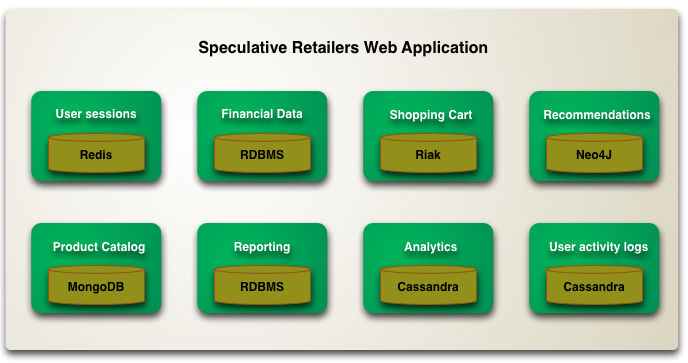
\includegraphics[scale=0.45]{obrazky/polygnot-persistance}
\par\end{centering}
\caption{Ukázka typů dat a jejich databází ve fiktivní aplikaci podle konceptu Polygnot Persistance \cite{fowlerpp}}.
\end{figure}

\begin{thebibliography}{10}
\bibitem{Thesis-templates}\emph{\LyX{} and \LaTeX{} Thesis Themplates}
{[}online]. {[}cit. 2008-09-28]. Dostupný z WWW: \url{http://www.thesis-template.com/}

\bibitem{Diplomka-v-LaTeXu}Pele,\emph{ Diplomka v \LaTeX{}u} {[}online].
{[}cit. 2008-09-28]. Dostupný z WWW: \url{pele.gzk.cz/node/37}

\bibitem{Jirkovy-stranky}Roubal, Jiří\emph{. Jirkovy stránky}~{[}online].
{[}cit. 2008-09-28]. Dostupný z WWW: \url{dce.felk.cvut.cz/roubal/}

\bibitem{Lyx-cesky}Vydra, Vítězslav.\emph{ Počeštění \LyX{}u}~{[}online].
2008 {[}cit. 2008-09-28]. Dostupný z WWW: \url{people.fsv.cvut.cz/~vydra/lyxcesky.htm}

\bibitem{Tex-Gyre}\emph{Písmo \TeX-Gyre}~{[}online]. {[}cit. 2008-09-28].
Dostupný z WWW: \url{www.gust.org.pl/projects/e-foundry/tex-gyre}

\bibitem{NeuesKapitel}\emph{Neues Kapitel-Layout}~{[}online]. {[}cit.
2008-09-28]. Dostupný z WWW: \url{www.thesis-template.de/archives/5#more-5}

\bibitem{Vavreckova}Vavrečková, Šárka. \emph{Úprava dokumentů}~{[}online].
{[}cit. 2008-09-28]. Dostupný z WWW:\url{axpsu.fpf.slu.cz/~vav10ui/obsahy/dipl/typografie.pdf}

\bibitem{diplPraceSLU}\emph{Zdroje informací pro diplomové práce,
SLU}~{[}online]. {[}cit. 2008-09-28]. Dostupný z WWW: \url{axpsu.fpf.slu.cz/~vav10ui/obsahy/dipl/typodipl.html}

\bibitem{V-cem}\emph{V čem napsat diplomovou práci}~{[}online].
{[}cit. 2008-09-28]. Dostupný z WWW: \url{www.student.cvut.cz/cwut/index.php/Diplomová_práce#V_.C4.8Dem_napsat_diplomovou_pr.C3.A1ci}

\bibitem{Menousek}Menoušek, Jiří. \emph{Jak (ne)napsat diplomovou
a dizertační práci}~{[}online]. {[}cit. 2008-09-28]. Dostupný z WWW:
\url{www.csmo.cz/other/dizert.php}

\bibitem{Polach}Polách, Eduard. \emph{Pravidla sazby diplomových
prací}~{[}online]. {[}cit. 2008-09-28]. Dostupný z WWW: \url{home.pf.jcu.cz/~edpo/pravidla/pravidla.html}

\bibitem{Citace}Farkašová, Blanka, Krčál, Martin. \emph{Projekt bibliografické
citace}~{[}online]. {[}cit. 2008-09-28]. Dostupný z WWW: \url{www.citace.com}.

\end{thebibliography}
~\\
Tento seznam literatury byl vytvořen přímo v Lyxu pomocí stylu ,,Bibliografie{}``
a generátoru citací~\cite{Citace}. Pořadí citací je takové, jak
je sami napíšeme.

\bibliographystyle{csplainnat}
\bibliography{bakalarka}
~\\
~\\
Tento seznam literatury byl vytvořen pomocí \BibTeX u s použitím
stylu \texttt{csplainnat}. Citace jsou automaticky seřazeny podle
abecedy.

\addcontentsline{toc}{chapter}{Literatura} 

\cleardoublepage{}

\appendix
\pagenumbering{Roman}\addcontentsline{toc}{part}{Přílohy}\thispagestyle{empty}  \renewcommand{\appendixname}{P\v{r}iloha}%%přílohy, číslování římskými


\part*{Přílohy}


\chapter[\noindent Souhrn výsledků testování]{\noindent Celkový souhrn výsledků testů}
\begin{table}[h]
\centering
\caption{Výsledky provedených měření}
\begin{tabular}{ | l | c | c | c | }
\hline
\multicolumn{4}{|c|}{Vložení 1000 dokumentů} \\ \hline
Testovací instance &MySQL&MongoDB server & MongoDB cluster \\ \hline
1 & 0,509s & 0,359s & 1,739s \\ \hline
2 & 0,474s & 0,297s & 2,397s \\ \hline
3 & 0,812s & 0,283s & 1,583s \\ \hline
4 & 0,608s & 0,331s & 2,229s \\ \hline
5 & 0,483s & 0,277s & 3,664s \\ \hline
Průměr & 0,598s & 0,309s & 1,987s \\ \hline
\end{tabular}
\end{table}

\begin{table}[h]
\centering
\begin{tabular}{ | l | c | c | c | }
\hline
\multicolumn{4}{|c|}{Vložení 10 000 dokumentů} \\ \hline
Testovací instance &MySQL&MongoDB server & MongoDB cluster \\ \hline
1 & 4,806s & 2,743s & 12,306s \\ \hline
2 & 4,992s & 2,824s & 12,116s \\ \hline
3 & 4,776s & 2,975s & 18,274s \\ \hline
4 & 5,136s & 2,906s & 20,981s \\ \hline
5 & 4,675s & 3,101s & 9,893s \\ \hline                                                                
Průměr & 4,877s & 2,909s & 15,918s\\ \hline
\end{tabular}
\end{table}

\begin{table}[h]
\centering
\begin{tabular}{ | l | c | c | c | }
\hline
\multicolumn{4}{|c|}{Vložení 100 000 dokumentů} \\ \hline
Testovací instance &MySQL&MongoDB server & MongoDB cluster \\ \hline
1 & 59,146s & 44,507s & 98,469s \\ \hline
2 & 60,604s & 40,318s & 112,192s \\ \hline
3 & 59,535s & 39,283s & 101,159s \\ \hline
4 & 63,080s & 35,214s & 132,715s \\ \hline
5 & 67,666s & 37,250s & 121,715s \\ \hline
Průměr & 62,006s & 39,315s& 113,294s\\ \hline
\end{tabular}
\end{table}

\begin{table}[h]
\centering
\begin{tabular}{ | l | l | l | l | }
\hline
\multicolumn{4}{|c|}{Získaní entity podle klíče} \\ \hline
Testovací instance &MySQL&MongoDB server & MongoDB cluster \\ \hline
1 & 0,822ms & 1,128ms & 0,661ms \\ \hline
2 & 1,885ms & 0,84ms & 0,701ms \\ \hline
3 & 1,282ms & 3,799ms & 0,432ms \\ \hline
4 & 4,448ms & 1,101ms & 0,867ms \\ \hline
5 & 1,745ms & 2,189ms & 0,611ms \\ \hline 
Průměr & 2,037ms & 1,812ms & 0,654ms \\ \hline
\end{tabular}
\end{table}

\begin{table}[h]
\centering
\begin{tabular}{ | l | l | l | l | }
\hline
\multicolumn{4}{|c|}{Získaní entity podle její vlastnosti} \\ \hline
Testovací instance &MySQL&MongoDB server & MongoDB cluster \\ \hline
1 & 3,385ms & 2,138ms & 0,347ms \\ \hline 
2 & 5,381ms & 0,869ms & 1,501ms \\ \hline
3 & 3,709ms & 3,291ms & 0,721ms \\ \hline
4 & 8,779ms & 1,929ms & 4,411ms \\ \hline
5 & 2,171ms & 1,621ms & 0,811ms \\ \hline
Průměr & 4,685ms & 1,969ms & 1,558ms \\ \hline
\end{tabular}
\end{table}

\begin{table}[h]
\centering
\begin{tabular}{ | l | l | l | l | }
\hline
\multicolumn{4}{|c|}{SELECT + FETCH jedné entity} \\ \hline
Testovací instance &MySQL&MongoDB server & MongoDB cluster \\ \hline
1 & 7,181ms & 4,833ms & 12,451 \\ \hline
2 & 14,051ms & 5,691ms & 5,001ms \\ \hline
3 & 25,001ms & 12,272ms & 7,852ms \\ \hline
4 & 11,991ms & 8,969ms & 4,503ms \\ \hline
5 & 12,591ms & 5,059ms & 9,276ms \\ \hline
Průměr & 14,162ms & 7,365ms & 7,816ms \\ \hline
\end{tabular}
\end{table}

\begin{table}[h]
\centering
\begin{tabular}{ | l | l | l | l | }
\hline
\multicolumn{4}{|c|}{SELECT + FETCH deseti entit} \\ \hline
Testovací instance &MySQL&MongoDB server & MongoDB cluster \\ \hline
1 & 22,438ms & 11,595ms & 19,468ms \\ \hline
2 & 17,319ms & 12,989ms & 24,155ms \\ \hline
3 & 12,180ms & 15,339ms & 17,154ms \\ \hline
4 & 17,792ms & 13,294ms & 20,006ms \\ \hline
5 & 9,469ms & 7,692ms & 26,978ms \\ \hline
Průměr & 15,839ms & 12,182ms & 21,552ms \\ \hline
\end{tabular}
\end{table}

\begin{table}[h]
\centering
\begin{tabular}{ | l | l | l | l | }
\hline
\multicolumn{4}{|c|}{Editace entity} \\ \hline
Testovací instance &MySQL&MongoDB server & MongoDB cluster \\ \hline
1 & 0,964ms & 1,656ms & 5,535ms \\ \hline
2 & 1,409ms & 1,706ms & 5,039ms \\ \hline
3 & 2,698ms & 5,131ms & 7,689ms \\ \hline
4 & 2,169ms & 3,091ms & 6,131ms \\ \hline
5 & 1,731ms & 1,566ms & 4,801ms \\ \hline
Průměr & 1,794ms & 2,630ms & 5,839ms \\ \hline
\end{tabular}
\end{table}

\begin{table}[h]
\centering
\begin{tabular}{ | l | l | l | l | }
\hline
\multicolumn{4}{|c|}{Přidání indexu na množinu miliónu záznamů} \\ \hline
1 & 24,027s & 23,952s & 38,729s \\ \hline
2 & 24.998s & 24,651s & 50,922s \\ \hline
3 & 22,441s & 23,417s & 40,431s \\ \hline
4 & 21,979s & 25,218s & 35,951s \\ \hline
5 & 22,504s & 26,251s & 46,145s \\ \hline
Testovací instance &MySQL&MongoDB server & MongoDB cluster \\ \hline
Průměr & 23,358s & 24,697s & 42,435s \\ \hline
\end{tabular}
\end{table}

\begin{table}[h]
\centering
\begin{tabular}{ | l | l | l | l | }
\hline
\multicolumn{4}{|c|}{Smazání záznamu } \\ \hline
1 & 85,288ms & 2,635ms & 5,089ms \\ \hline
2 & 38,568ms & 2,546ms & 7,995ms \\ \hline
3 & 37,140ms & 10,523ms & 6,243ms \\ \hline
4 & 82,751ms & 16,577ms & 9,155ms \\ \hline
5 & 23,151ms & 22,194ms & 4,789ms \\ \hline
Testovací instance &MySQL&MongoDB server & MongoDB cluster \\ \hline
Průměr & 53,379ms & 10,895ms & 6,654ms \\ \hline
\end{tabular}
\end{table}



\end{document}
